\chapter{Lab 6\&7}
\setcounter{TASignatures}{0}
\setcounter{AsideCounter}{0}

\section{Introduction}
    \vspace{0.1em}

    \textbf{In this lab you gain experience with:}
    \begin{enumerate}
        \item Editing HMI applications
        \item Sending information from the HMI to the PLC
        \item Displaying information from the PLC on the HMI
        \item More timers
    \end{enumerate}
    
    \textbf{You will also gain experience with the following HMI objects:}
    
    \begin{enumerate}
        \item Momentary Buttons
        \item Numeric Entry
        \item Numeric Display
        \item Text Boxes
        \item Multi-State Indicators
    \end{enumerate}

\subsection{Lab Files}

Go to iLearn and download the PLC and HMI files for this lab to the PC. Then download the PLC project to the PLC and the HMI application to the HMI. 

\subsection{Acceptable Instructions}

You may have previous experience with PLCs and that is great! However, you are only allowed to use the instructions that we have covered thus far in the lab. So, if you have experience already, consider it a challenge to restrict yourself to only use the instructions that have been covered thus far in lecture to solve the problem!

\subsection{Lab agreement}

The planning of a program is often a very social activity, however the actual writing of the code is always an individual pursuit. In this class it is very much the same. Students are welcome to verbally assist each other, but each person is required to write their own code and personally complete each lab. In this way each student will gain valuable experience with programming PLCs. 

\textbf{The undersigned person guarantees that any and all work demonstrated to the TA in regard to this lab is a result of their own work with no unauthorized help.}

\signatureSlot{Student}



\section{Editing the HMI Application}

In lab 0 you gained experience with downloading an existing HMI application to the HMI. At this point you should be familiar with how to set the IP address and download to the appropriate HMI. 

In this lab you will be editing an existing HMI application and programming the PLC so that both meet the requirements laid out in each of the lab exercises below. 

Each of the HMI objects necessary to complete this lab has been demonstrated in video lecture 6. Refer to the lecture if you are unsure how to create any of these objects. The video lecture also demonstrates the process to connect these objects with a tag in the PLC, create a runtime application, and download the runtime application to the HMI. The information in this section below is intended to reiterate what has already been demonstrated. 

\aside{The HMI interacts with the PLC by reading and writing values in PLC tags. When a button is pressed, the HMI typically writes a true value into some boolean tag. When the button is released, the HMI writes a false value into the tag. Similarly, when a number is entered into a numeric entry field, the HMI sets the value of an associated tag in the PLC to the value which was typed.}


\subsection{General Process to Developing an HMI application}

Here a general approach to developing an HMI application is given. This approach assumes that you have already have an HMI application file and with the settings chosen appropriately for the HMI to which the application will be downloaded. In this class, that will always be the case.

\subsubsection{Start by creating your tags in the PLC}
The HMI software is able to detect the available tags that are present in the PLC. This makes associating HMI objects with PLC tags easier. However, for the HMI software to accomplish this, the tags must already exist in the PLC. For this reason, \textbf{before you start developing the HMI application}, you should first create any tags that will be used in the HMI application and download the tags to the PLC. It is not necessary that all your PLC code be written, only that the tags you intend to use in the HMI are created in the project and downloaded.

\aside{In general it is best to keep your tags very organized. Often this involves using local tags only, with very few exceptions. However, in this introductory course, tag location is not emphasized.}

\subsubsection{Adjust the HMI communication setup}
For the HMI application and the PC software to see the tags which are in the PLC, you must complete the HMI communication setup as you typically would before downloading a project to the HMI at the beginning of lab. 


\subsubsection{Creating the object(s)}
After you have created and downloaded the tags you intend to use to the PLC and have successfully setup the communication for the HMI, it is time to begin making edits to the HMI application. At this point you should create the on screen objects that you need. 

\subsubsection{Connect the object to the desired PLC tag}
After you have created an object, \textbf{right click} the object and open the \textbf{properties menu}. Here, select \textbf{connections}. Depending on the object you have created, there may be multiple connection options. The options for a momentary pushbutton are shown in \figureautorefname \ref{fig:ConnectionMomentary}. 

In \figureautorefname \ref{fig:ConnectionMomentary} notice the column labeled "Tag" to the right of the center. The ellipses is clickable and gives a list of available tags.  

\begin{figure}[h]
\centering
\textbf{Connection options for Momentary Pushbutton}\par \medskip
\frame{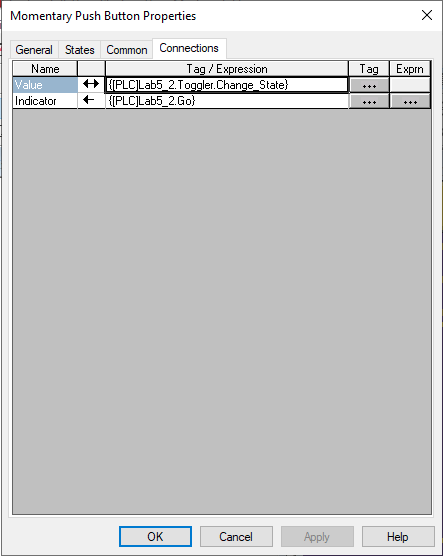
\includegraphics[width=3in]{ConnectionMomentary}}
\caption{Count up instruction}
\label{fig:ConnectionMomentary}
\end{figure}

After clicking the ellipses, a menu similar to the one shown in \figureautorefname \ref{fig:TagSelection} should appear. Select a folder on the left and the available tags in that folder will appear on the right. In \figureautorefname \ref{fig:TagSelection}, the folder called "Program.MainProgram" was selected. 

Note: Clicking the plus button beside a tag folder will show any nested folders. However, to see the tags in a folder, the folder itself must be highlighted.

Note: It may be that the HMI software (FactoryTalk View Studio) has not scanned the PLC to get the most updated list of available tags. If you don't see the tags you have created, click the Refresh All Folders button shown in the bottom left of \figureautorefname \ref{fig:TagSelection}. If you still can't find your tags, follow the steps below:

\begin{samepage}
\begin{itemize}
    \item Make sure you have downloaded the tags to the PLC
    \item Ensure that the PLC is in Run mode
    \item Make sure that the communication setup in the HMI has been completed
\end{itemize}
\end{samepage}

\begin{figure}[h]
\centering
\textbf{Tag selection}\par \medskip
\frame{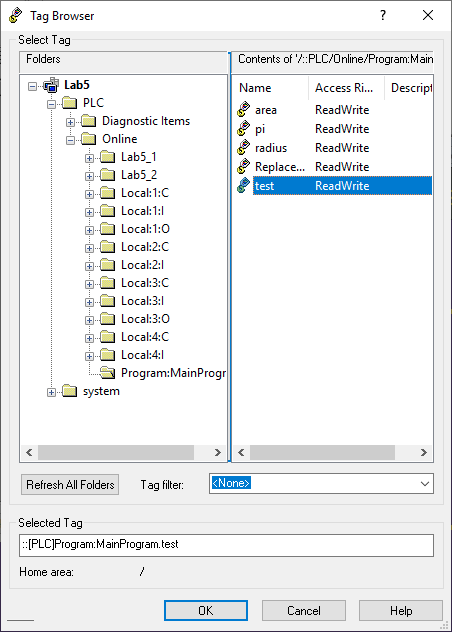
\includegraphics[width=3in]{TagSelection}}
\caption{Tag Selection}
\label{fig:TagSelection}
\end{figure}

\subsubsection{Create the Runtime Application}
When you have completed your HMI edits and are ready to download the application, it is time to create the runtime application. 

Go to the Application menu and select Create Runtime Application. In the dialog window that appears, select save. 

\subsubsection{Download the HMI application}
Finally, it is time to download the HMI runtime application. Use the transfer utility as you have previously to transfer the runtime to the HMI.



\section{Challenge - StopWatch}
(Notice that there is no associated object for this lab. You must create all the necessary tags and HMI objects to fulfill the requirements outlined in this exercise. Make sure that the HMI page you make looks professional.)
\\

Another weekly challenge from the competition for which you signed up! This week you will have to edit both the provided HMI and PLC files to accomplish the functionality.

Write a ladder logic program that will act as a stopwatch. Create a boolean tag called \verb|Start| that will act as the start button for the stopwatch. The \verb|Start| tag must be associated with a button labeled start on the HMI. Your PLC logic must calculate the time which has elapsed sense the \verb|Start| button was pressed. 

Further, you must create a pause button on the HMI that is connected to a boolean tag in the PLC that you must also create. The tag should be named \verb|Pause|. Your PLC ladder logic must implement pause functionality so that the stopwatch is paused after the \verb|Pause| signal becomes true and may be continued by pressing start again. 

Also, you must create a boolean tag in the PLC called \verb|Reset|. This tag must be associated with a button on the HMI with the same name. If the \verb|Reset| button is pressed then the timer should be reset to zero and stopped. 

Finally, the timer will track the elapsed time in milliseconds. You must take the elapsed time in milliseconds and convert it to seconds and minutes. The seconds and minutes should be displayed on the HMI.


\subsection{Hints}

The general logic has already been described.

You will need to create a tag of type TIMER. Create the tag and give it the name \verb|Stopwatch_TMR|. Use one of the two timer instructions that have been discussed in lecture. For information regarding the two timer instructions, refer to the Allen Bradley instruction manual on iLearn.

You will need to create the tags listed in \tableautorefname \ref{Table:Lab7_1Tags} in the PLC and use them appropriately in the HMI. You may create other tags as necessary.

\aside{The accumulated time is stored in the .ACC attribute of the TIMER tag. The value stored in the .ACC attribute is the elapsed time in milliseconds. To get the elapsed time in seconds and minutes is a matter of simple arithmetic.}

\subsection{The Inputs and Outputs}

To access any of the tags that you create, use the tag name without any prefix. This is different from the method used to access tags that were already provided in previous labs.

\begin{table}[h]
\centering
\caption{Tags you will create in Lab7\textunderscore 1\\ (Create others as necessary)}
\label{Table:Lab7_1Tags}
\begin{tabular}{c c}
\toprule
Tag Name & Data Type\\
\midrule
\verb|Start| & BOOL \\
\verb|Pause| & BOOL\\
\verb|Reset| & BOOL\\
\verb|Seconds| & Dint\\
\verb|Minutes| & Dint\\
\verb|Stopwatch_TMR| & TIMER\\
\bottomrule
\end{tabular}
\end{table}

Write the appropriate logic under the associated rung in the PLC file.

\TASignatureSlot



\section{Blinking Lights}
(Notice that there is no associated object for this lab. You must create all the necessary tags and HMI objects to fulfill the requirements outlined in this exercise. Make sure that the HMI page you make looks professional.)
\\

You have again been contacted by Transmission Makers of America to do some contract work for them. They want you to display a light (indicator) on the HMI and make the light (indicator) blink. 

A blinking light is actually a square waveform. So, they want to be able to enter the period in milliseconds of the blinking pattern. They also want to be able to enter the duty cycle in percentage on the HMI. So, if they enter 200 for the period and 50 for the duty cycle, it should produce a light blinking pattern like the one shown in \figureautorefname \ref{fig:Blink20050}. The Light has a "high" value on the graph, when the light is on, on the HMI.

\begin{figure}
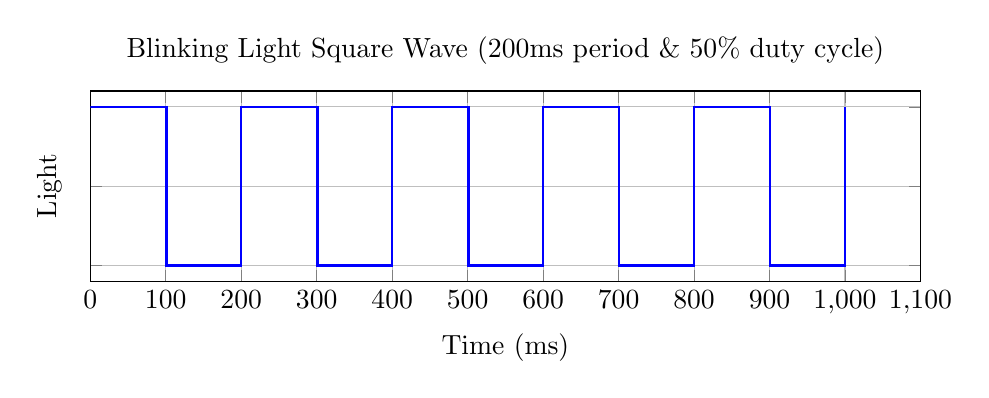
\begin{tikzpicture}
\begin{axis}[grid=both,xmin=0,width=\columnwidth,height=4cm,
title={Blinking Light Square Wave (200ms period \& 50\% duty cycle)},xlabel={Time (ms)},ylabel=Light,
yticklabels={,,}]
\addplot+[thick,const plot, no marks,samples at={0,1,...,1000}] {(mod(x,200)>(200*0.5)?0:1)};
\end{axis}
\end{tikzpicture}
\caption{Pattern on light with a 200ms period and 50\% duty cycle}
\label{fig:Blink20050}
\end{figure}

If the user were to type 400 for the period and 20 for the duty cycle, the PLC should cause the indicator on the HMI to blink in a pattern like that shown in \figureautorefname \ref{fig:Blink40020}.

\begin{figure}
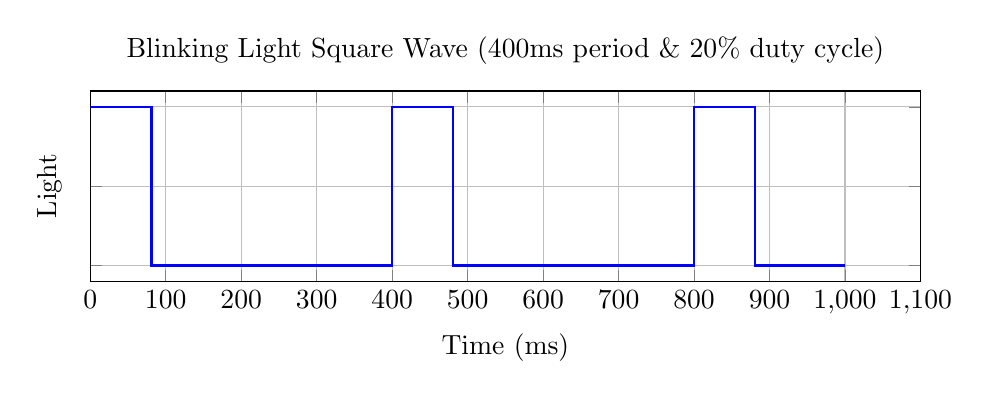
\begin{tikzpicture}
\begin{axis}[grid=both,xmin=0,width=\columnwidth,height=4cm,
title={Blinking Light Square Wave (400ms period \& 20\% duty cycle)},xlabel={Time (ms)},ylabel=Light,
yticklabels={,,}]
\addplot+[thick,const plot, no marks,samples at={0,1,...,1000}] {(mod(x,400)>(400*0.2)?0:1)};
\end{axis}
\end{tikzpicture}
\caption{Pattern on light with a 400ms period and 20\% duty cycle}
\label{fig:Blink40020}
\end{figure}

Note: In this exercise you decide what tags to create and what to name them. Make sure that you name them appropriately so that you (and others that may come behind you) know what the tags are meant to do.

\subsection{Hints}

To implement blinking lights, you will have to use timers. You will most likely need two timers. One for the on time, and one for the off time. Calculate the amount of on and off time using the period length and the duty cycle.

Problems like this are best attacked one step at a time. So, I would recommend the following decomposition:

\begin{itemize}
    \item Create the tag which you will associate with the hmi light in the PLC
    \item Create the multi-state indicator in the HMI, associate it with the PLC tag, and download the application
    \item Test the tag in the PLC by manually toggling it to see that the light blinks as it should
    \item Create timers and logic in the PLC to make the light blink
    \item Create the tags in the PLC for the desired duty cycle and blink period
    \item Write the logic to calculate the appropriate on and off time based on the period and duty cycle
    \item Test the duty cycle and period logic in the PLC manually by entering different values in the monitor tab of the tags menu
    \item Create numeric entry objects in the HMI and associate them with the duty cycle and period tags in the PLC
    \item Test the overall functionality
\end{itemize}

\TASignatureSlot



\section{C. A. L. See You Later.}
(Notice that there is no associated object for this lab. You must create all the necessary tags and HMI objects to fulfill the requirements outlined in this exercise. Make sure that the HMI page you make looks professional.)
\\


The grocery store manager has contacted you about doing some further work. They have been running into situations where they need a general purpose calculator available to all employees. They have purchased calculators in the past but they always manage to get lost. So, the manager wants you to add a calculator to the PLC and HMI that you have previously programmed. This way the calculator can't be lost!

The manager wants to be able to enter two operands on the HMI, \verb|operandA| and \verb|operandB|, and have the result of the calculation displayed in a third numeric display field on the HMI. The calculator must be able to multiply, divide, add, and subtract. There should be a button for each of these operations on the HMI that will apply the desired operations to the operands and display the result.

So, if a user enters 5 into the numeric entry field for \verb|operandA| and 3 into the numeric entry field for \verb|operandB| and then presses the button for multiply, the number 15 will be displayed in the numeric display field for the result. 

 
\subsection{From Functional Description to Code}


Typically, when a client specifies their desired functionality, the description will not be complete. Almost certainly they will not tell you how to implement the functionality they desire. So, in this problem, part of the exercise is figuring out what tags you will need to create in the PLC to make the desired HMI functionality possible. With that in mind, spend some time ensuring that you understand exactly how the calculator should work. Then consider how to accomplish the desired functionality using ladder logic and the HMI. After you have developed a plan, begin to program.

\TASignatureSlot



\section{What's the combination again?}
(Notice that there is no associated object for this lab. You must create all the necessary tags and HMI objects to fulfill the requirements outlined in this exercise. Make sure that the HMI page you make looks professional.)
\\


The grocery store manager had a second request. The store has a safe and every night all the large bills in the cash registers are removed and stored in the safe. But there are several department managers that need to be able to access the safe, some of which aren't very good at remembering the 7 number combination. The result is that every night the store manager is called and asked for the combination.

To fix this problem the manager has decided that they want you to add a screen to the HMI that will allow the department managers to type in a shorter pin number and press a button labeled ``Show Combo". After typing in the correct pin number and pressing the button, the safe combination will be displayed one number at a time, with each number being displayed for 3 seconds.

The manager has required that the pin number be 118. The safe combination is 3, 5, 8, 13, 21, 34, 55, 89. 

\aside{This problem has a set of things that must be done in the same order every time. These sequential functions are easier to implement if you use a structured bit latch sequence.}


\subsection{From Functional Description to Code}

Typically, when a client specifies their desired functionality, the description will not be complete. Almost certainly they will not tell you how to implement the functionality they desire. So, in this problem, part of the exercise is figuring out what tags you will need to create in the PLC to make the desired HMI functionality possible. With that in mind, spend some time ensuring that you understand exactly what the manager wants. Then consider how to accomplish the desired functionality using ladder logic and the HMI. After you have developed a plan, begin to program.

\TASignatureSlot